"To improve and expand urban disaster facilities and plans, new urban parkland should be infrastructural and multi-functional; they should be used as a daily part of urban life while maintaining the mechanisms needed to support local community and to respond to natural or unexpected disasters."---Noboru Masuda (2014)

This chapter will cover a brief history of city parks, especially as they have related to times of urban crisis and disaster. From the spread of cholera in the 1820s, to the most recent global public health crisis that began in 2020, city parks are an important part of the urban infrastructure. This section will provide historical context for the evolution of city parks and help set the stage for how parks might need to change in response to the COVID-19 pandemic.\\
 
\begin{multicols}{2}

\section{City parks} 
Originally, green spaces in many European cities and throughout Japan were not public spaces, instead reserved for the wealthy and the elite \cite{havens_parkscapes_2011}\cite{jones_equity_2009}. The establishment of city parks began around the same time urban life was changing dramatically due to the Industrial Revolution. Industrialization, overcrowdedness, and infectious diseases made cities unhealthy and unpleasant, and city parks were seen as a solution to these problems \cite{malchow_public_1985}\cite{jones_lungs_2018}. 

Across Europe, many green spaces were owned by royal families until the nineteenth century. One of the earliest examples of a green space created for the public was in Paris in 1605 CE, when the king had the Place de Vosges constructed as a place for respite from the overcrowded city \cite{jones_lungs_2018}. In London, several royal parks transitioned from royal hunting grounds to public space, including Hyde Park in 1637 \cite{jones_lungs_2018}. Later, Birkenhead Park in England opened in April 1847---now known to be the first publicly funded urban park \cite{tate_great_2013}. In 1943 the County of London Plan aimed to provide more green space to improve the health of people \cite{hill_forshaw_2005}, showing the connection between public health and parks continued into the twentieth century.

In the US in the 1850s, New York City was densely crowded and infected with cholera, tuberculosis, and other diseases, according to Cranz (1989). Public health officials argued for the establishment of Central Park "because they observed that clean air helped reduce the spread of disease" \cite{cranz_politics_1989}. Early twentieth century then saw a rise in neighborhood parks and playgrounds to provide a place deemed as safe for children to play. Perhaps because parks were considered public space, civic uses were commonplace, such as army recruitment in the 1920s, and during the Great Depression parks were used recreation as a means of social control by diversion from issues such as unemployment \cite{cranz_politics_1989}.

City parks in Japan were influenced by those in Europe and the US in the nineteenth century around the time of the Meiji Restoration. According to Havens (2011), Edo delegates were sent from Japan to Europe and the United States in 1860 to "investigate the secrets of capitalist modernity," one of the findings being parks in the US, England and France. Before this visit, much green space already existed in Japan in the form of temples and gardens, but like many other countries, it typically belonged to the high-ranking and wealthy \cite{havens_parkscapes_2011}. The advocates of the early city parks in Japan saw the many benefits of the open spaces: recreation, disaster relief, political control, hygiene, and curbing infectious diseases \cite{havens_parkscapes_2011}. 

In each of the cities studied, city parks have been associated with times of national crisis since their inception as public space. Shortly after Hyde Park opened to the public in the seventeenth century, the grounds were used for city residents to escape the plague \cite{noauthor_history_nodate}. In the mid-nineteenth century, authorities in both England and US sought parks as the solution to "population growth, hygiene, mortality and communicative disease" with Victoria Park in London opening in 1845 to stop spreading epidemics \cite{jones_lungs_2018}. Also in London, to prepare for air raids during World War II, trench shelters were built in parks and open spaces \cite{ainsworth_geophysical_2018}. 

An example of the relationship between parks and disasters in the US is the use of Golden Gate Park in the aftermath of the 1906 San Francisco earthquake as a place for the displaced to set up refugee camps \cite{cranz_politics_1989}. During the Great Depression, recreation programs were created as relief for the unemployed in San Francisco, and in New York, Works Progress Administration (WPA) workers were assigned to park construction and maintenance projects during this same time \cite{cranz_politics_1989}. During World War II, parks hosted first aid classes, provided space for barracks and other military activities, and operated as community gardens for vegetables and flowers \cite{cranz_politics_1989}. 

\end{multicols}

\begin{figure}[h]
  \centering
  \vspace{8pt}
  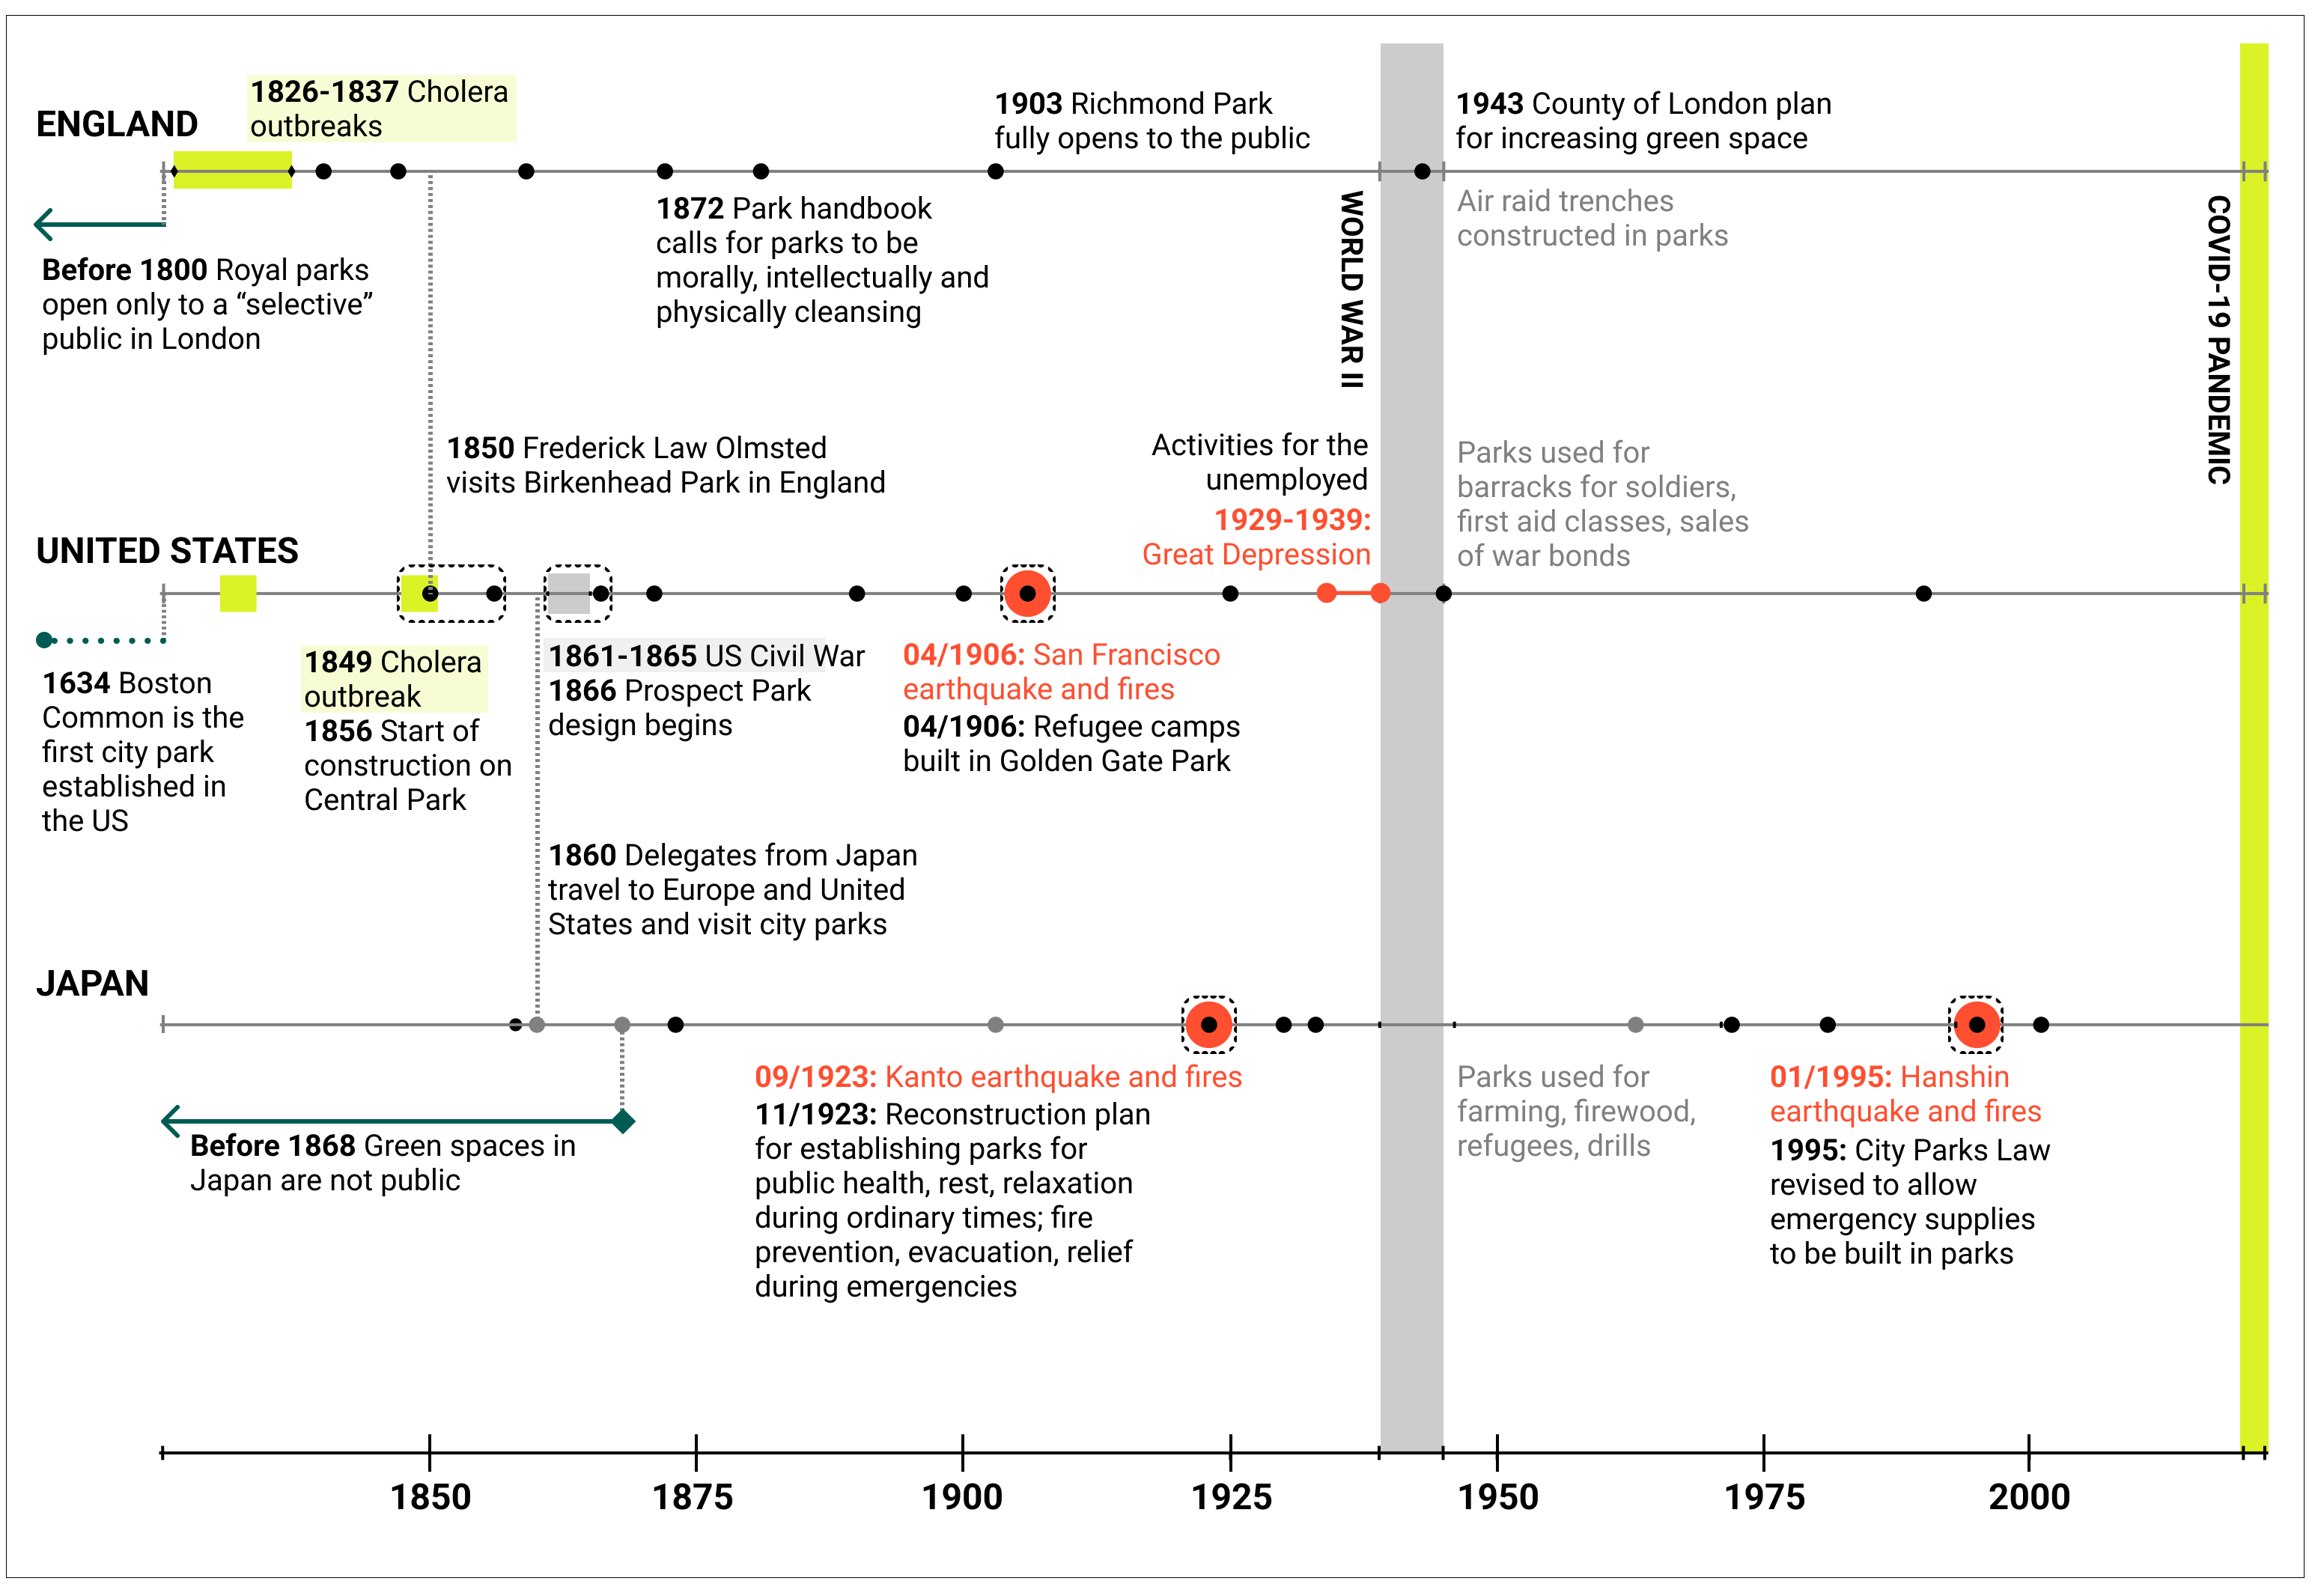
\includegraphics[width=1.0\textwidth]{images/crisis/timeline.png}
  \captionsetup{width=1.0\linewidth}
  \caption[Timeline diagram]{Comparative timeline showing the history of city parks and disaster events for England, the United States and Japan.}
  \label{fig:timeline}
\end{figure}\par

\begin{multicols}{2}

In Tokyo, parks are closely tied to the disasters that have impacted the city. After the 1923 earthquake and fire, the government of Tokyo created a design plan for the city which used public parks and open spaces as firebreaks and refuge areas after a seismic event \cite{masuda_disaster_2014}. The reconstruction plan of November 1923 encouraged the establishment of parks for public health, rest and relaxation during ordinary times, and in the case of an emergency, for fire prevention, evacuation and relief \cite{havens_parkscapes_2011}. During World War II, parks not only served as firebreaks, but also housed soldiers in training, were used for farming and firewood, as refuge for the homeless, and more \cite{havens_parkscapes_2011}. Masuda (2014) explains that the urban park as a disaster refuge "should include a warehouse, earthquake-proof water tank, radio broadcasting facilities, helicopter pad, and fire fighting facilities" \cite{masuda_disaster_2014}. More recently, the benefits of parks include air quality improvement, serving as windbreaks and helping to reduce global warming by absorbing carbon dioxide \cite{havens_parkscapes_2011}.

Figure \ref{fig:timeline} shows a comparative timeline of the history of city parks and disaster events for England, the United States and Japan. There are clear influences between the three countries in this study regarding park implementation and design. Frederick Law Olmsted visited Birkenhead Park in England in 1850 CE before designing Central Park in New York in 1866 CE. Around the same time, delegates from Japan visited cities in Europe and the United States, bringing back to Japan the inspiration to build city parks \cite{havens_parkscapes_2011}.

From the perspective of governmental agencies, incentives to create and maintain city parks across time, geography and culture, are for the perceived notions of public health and social control, and for encouragement of leisure and recreation \cite{jones_lungs_2018}\cite{cranz_politics_1989}\cite{havens_parkscapes_2011}. The initial movement to create public parks in cities came as a response to the overcrowdedness which led to outbreaks of cholera and other diseases. Then, as wars erupted, natural disasters occurred, and eventually the occurrence of the recent pandemic, parks have been utilized to protect city residents.

\section{Crisis management}
Wisner and Adams (2002) write about emergency response strategies for the protection of the people and the environment in emergencies and disaster situations. The authors differentiate three phases as planning, prevention, preparedness and mitigation; emergency response; recovery, rehabilitation and reconstruction to promote sustainable development and, further, the authors express the importance of preparing for future disasters during "normal" times \cite{wisner_environmental_2002}.

The top diagram in Figure \ref{fig:crisis_management} shows the disaster management cycle from Wisner and Adams (2002), and then further adapts the diagram to express the disaster response cycle in relation to city parks. The middle diagram shows an impact as an earthquake, fire, war, or pandemic. As discussed previously, there are many examples across time and geography where city parks were used in response to a disaster. This includes evacuation and refugee centers after earthquakes and for farming or army training during a war. After each disaster and subsequent new uses, it is typical for legislation to be passed to improve existing parks or add new parks to better serve a city in the face of the next disaster. 

Amid the recent COVID-19 pandemic, city parks were used across the world for people to exercise, enjoy nature, socialize with friends despite the ongoing spread of disease \cite{bereitschaft_how_2020}. The bottom image in Figure \ref{fig:crisis_management} represents the response and mitigation efforts with the pandemic as the disaster impact event. The initial response to the spread of COVID-19 included lockdowns, cancelled events, and stay-at-home orders which restricted residents from leaving their homes except for "essential" activities \cite{storr_essential_2021}. As more information about the disease was understood, the public health response transitioned from the emergency response to recommendations for how to live with the spread of disease. Some of the resulting recommendations included masking requirements in public spaces, resumed service of public transportation, and the encouragement of low-risk social gatherings in outdoor spaces. 

Using the past disaster impacts and resulting changes in planning policy to better prepare city parks for future disasters, the research that follows will try to determine what might be changed to prepare three city parks for the next pandemic.

\end{multicols}

\newpage
\null
\vfill
\begin{figure}[H]
  \centering
  \captionsetup{width=0.9\textwidth}
  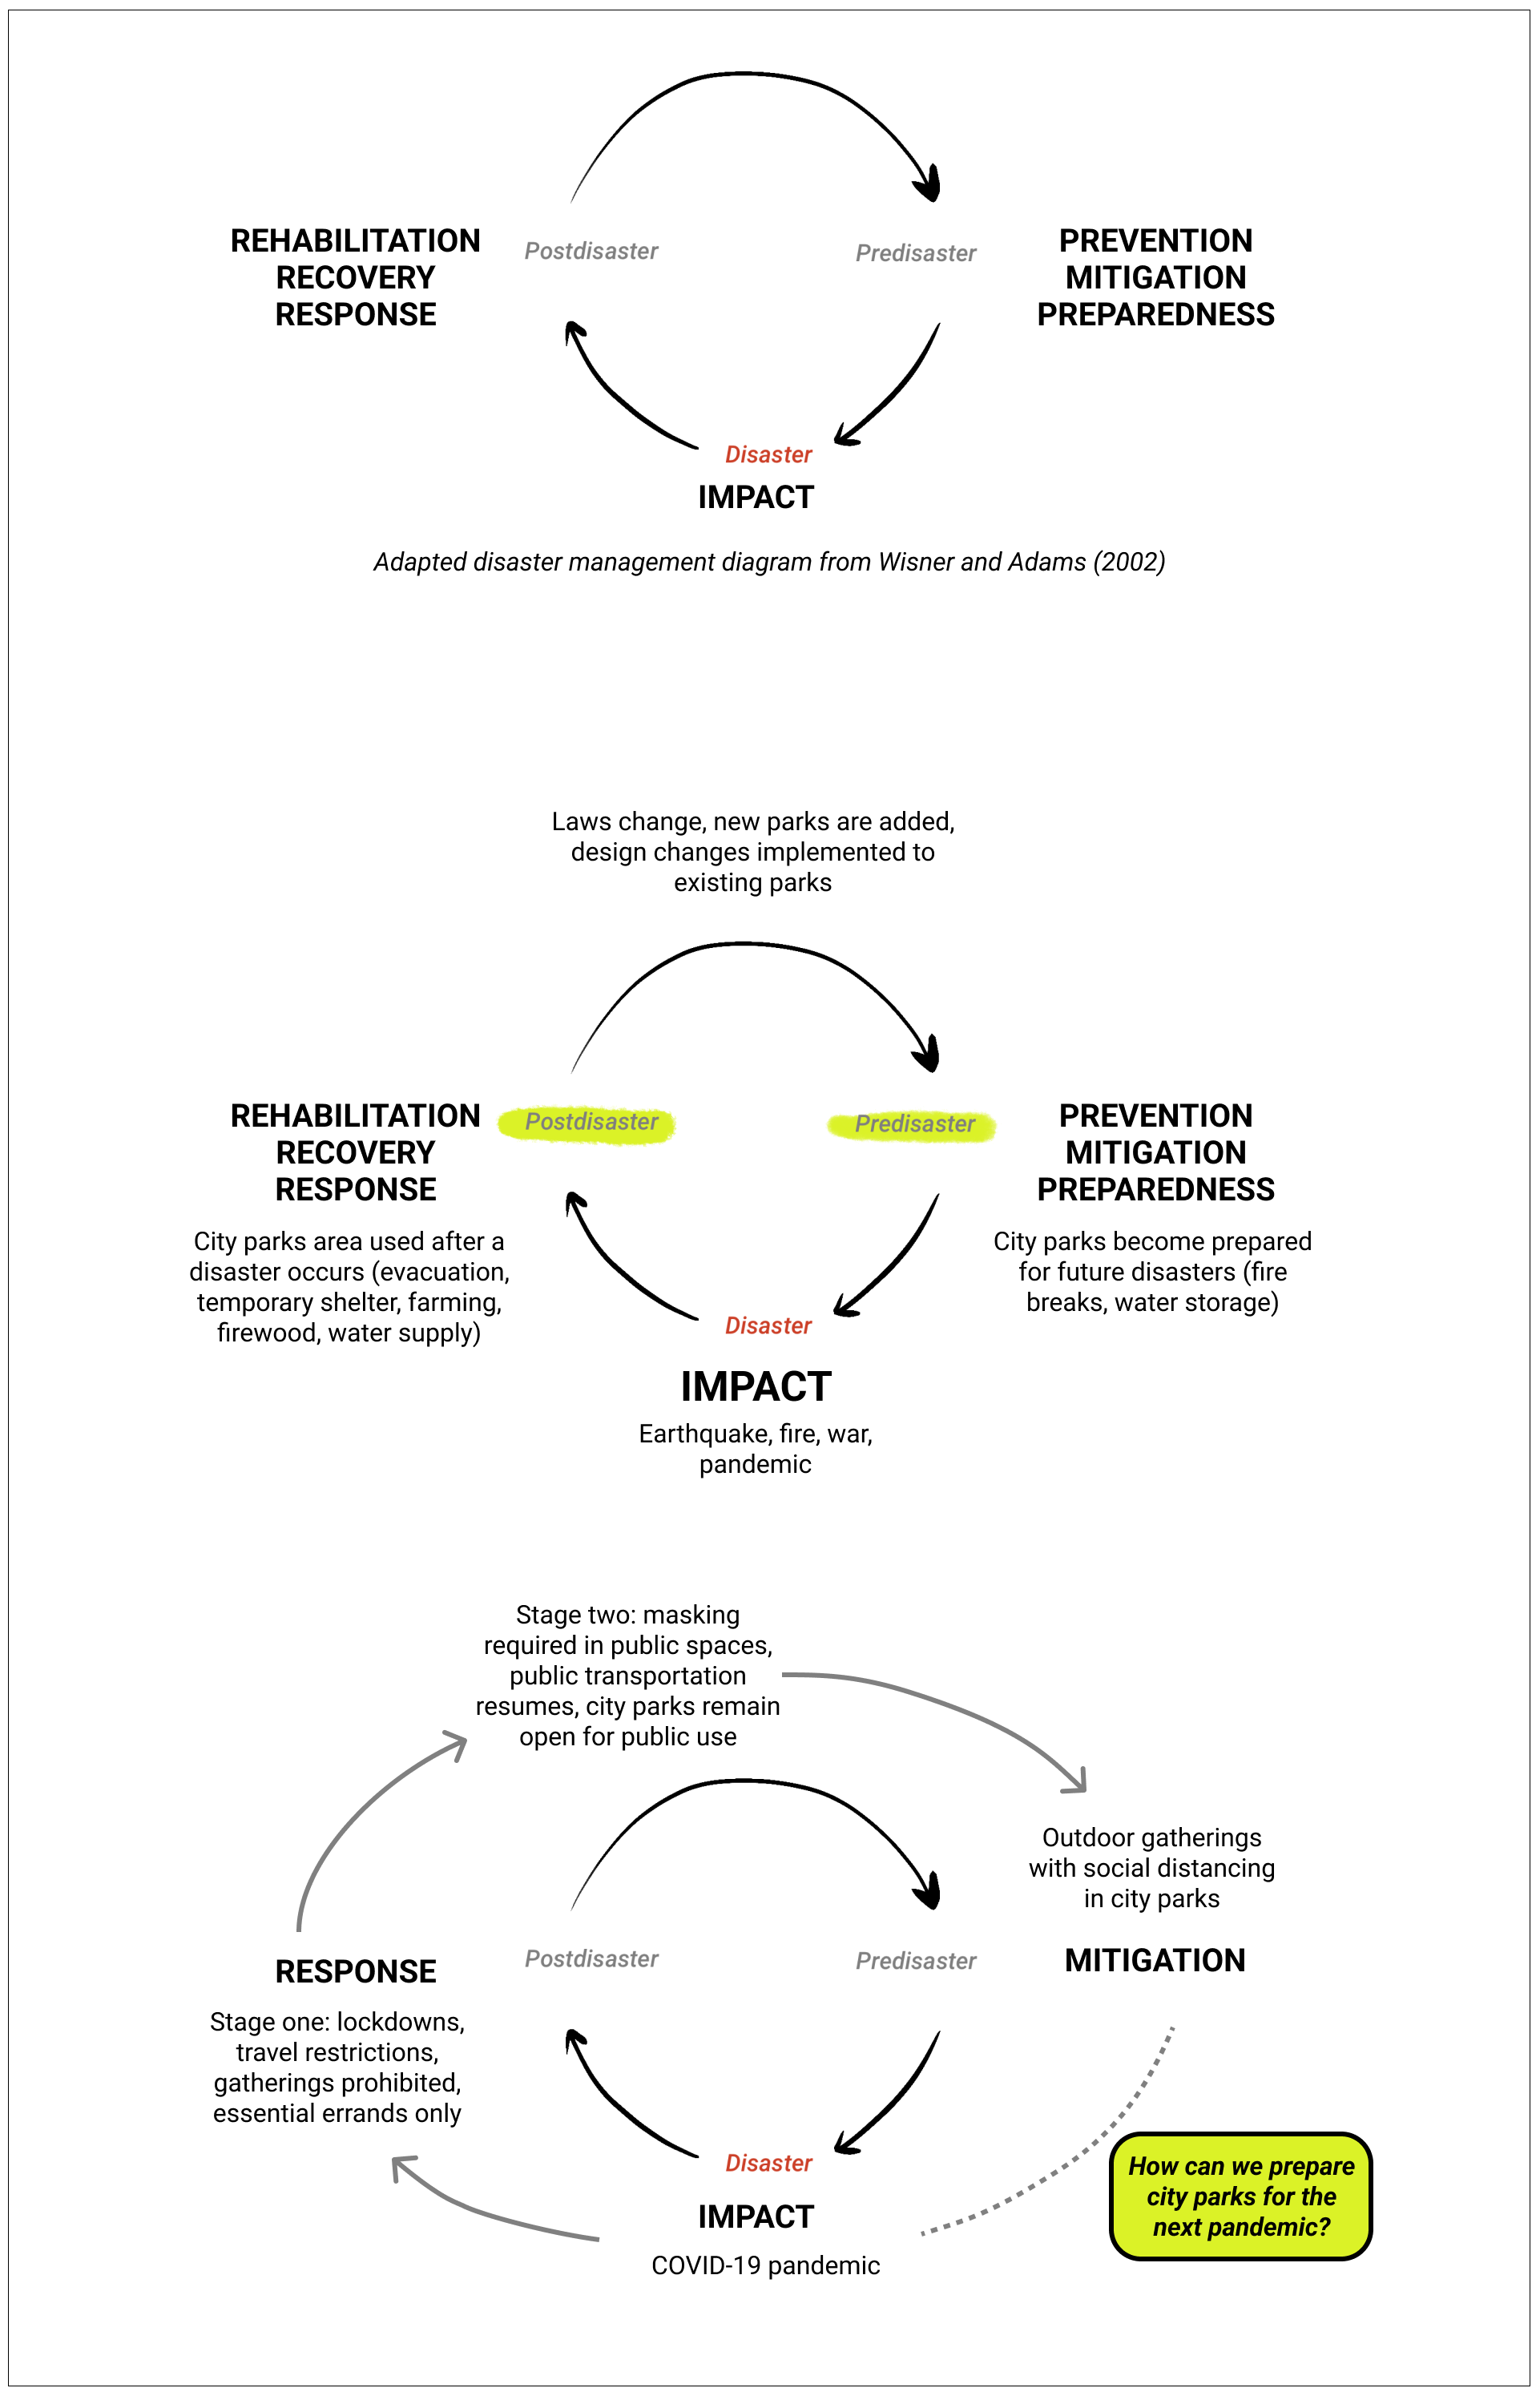
\includegraphics[width=0.9\textwidth]{images/crisis/crisis_management.png}\par\hspace{3pt}
  \caption[Crisis management diagram]{Top diagram: disaster management cycle, adapted from Wisner and Adams (2002) \cite{wisner_environmental_2002}; middle diagram: disaster management cycle relating to city park evolution; bottom diagram: disaster management cycle with COVID-19 as the disaster impact.}
  \label{fig:crisis_management}
\end{figure}

